% Made up for the tikra benchmark.
% The Petersen graph: an outer pentagon, an inner pentagram, and the five spokes between them.
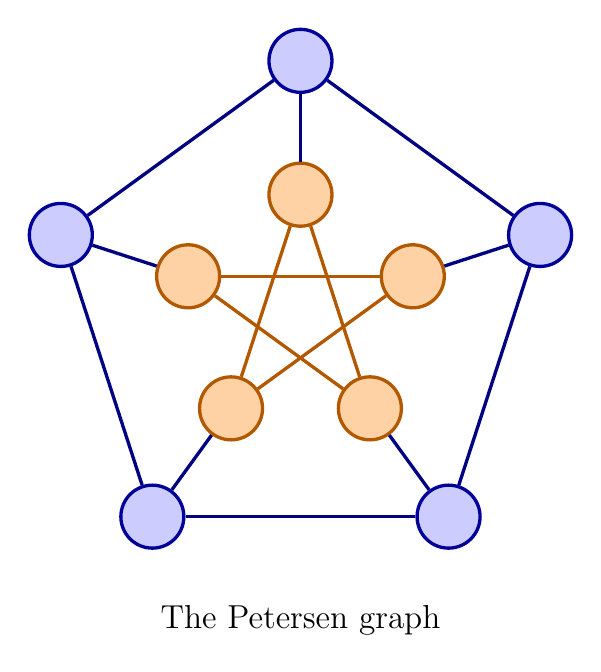
\begin{tikzpicture}[vertex/.style={circle, draw=blue!60!black, fill=blue!20, very thick, minimum size=8mm},
    every edge/.style={draw, very thick, blue!50!black}]
  \foreach \i in {0,...,4} {
    \node[vertex] (o\i) at (90+72*\i:3.2) {};
    \node[vertex, fill=orange!35, draw=orange!70!black] (n\i) at (90+72*\i:1.5) {};
  }
  \foreach \i [evaluate=\i as \j using {int(mod(\i+1,5))}, evaluate=\i as \k using {int(mod(\i+2,5))}] in {0,...,4} {
    \path (o\i) edge (o\j)
          (o\i) edge (n\i)
          (n\i) edge[orange!70!black] (n\k);
  }
  \node[font=\large] at (0,-3.9) {The Petersen graph};
\end{tikzpicture}
